\section{Proposed NeST-Com Framework}
\subsection{Next-Scale Representation and Digital Frame}
\begin{figure*}[t]
\centering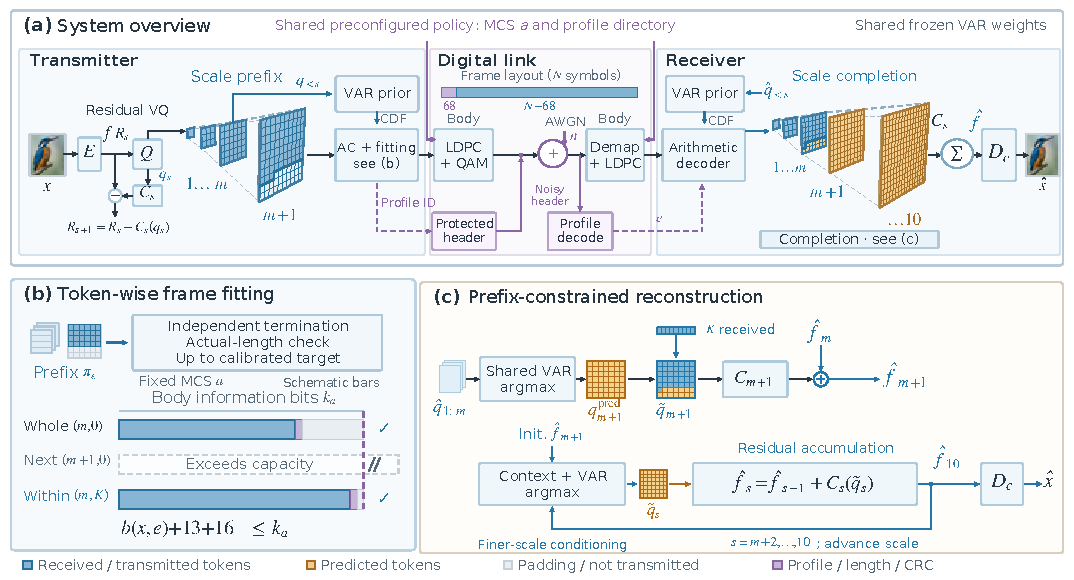
\includegraphics[width=\textwidth]{figure1_final.pdf}
\caption{NeST-Com. (a) The shared policy fixes the MCS and profile directory; the protected profile selects the endpoint. VAR and known coarse tokens provide coding probabilities. (b) Independently terminated prefixes fit the actual capacity below the target; bars are schematic. (c) Received tokens overwrite boundary predictions. Recursive state updates accumulate residuals and condition each finer scale before decoding. Unreceived boundary positions retain their coarse-conditioned predictions.}
\label{fig:system}
\end{figure*}
We transmit $x\in[0,1]^{256\times256\times3}$ using $N$ complex symbols over AWGN,
\begin{equation}
y=s+n,\quad n\sim\mathcal{CN}(0,\sigma^2 I_N),\quad
\mathrm{SNR}=10\log_{10}(E_s/\sigma^2),
\label{eq:channel}
\end{equation}
with nominal $E_s=2$. TX uses the frozen policy for its design SNR; RX uses the actual noise variance for LLRs. Digital constellations have average energy two without per-frame renormalization. A 12-bit profile ID, CRC16, and terminated rate-1/2 convolutional code occupy 68 rotated-BPSK symbols $\{\pm(1+j)\}$. Under a preconfigured policy, both terminals know the MCS and profile directory; the 12-bit profile identifies the endpoint within that directory. The remaining $N-68$ symbols carry the LDPC-coded body, with public frame-dependent scrambling after rate matching and inverse scrambling before decoding. Continuous JSCC data are normalized per image to energy two; required side information is paid within $N$.

The frozen VAR tokenizer produces ten residual token maps $q_s$, with side lengths $(1,2,3,4,5,6,8,10,13,16)$ and a 4096-entry codebook~\cite{var}. Write $L_s$ for the number of positions and $C_s$ for codebook lookup, resizing to the full latent grid, and the scale-dependent residual transform. The latent sum $\sum_s C_s(q_s)$ progressively refines a full-field description. Decoder $\Dc$ is adapted on 20\,000 ImageNet training images using MSE plus $0.1$ LPIPS, then frozen. The continuous/quantized/prefix-completed training mixture is specified in Supplement~S1. The null-class VAR-d16 prior factorizes as
\begin{equation}
p_\theta(q_s\mid q_{<s})=\prod_{i=1}^{L_s}p_\theta(q_{s,i}\mid q_{<s}).
\label{eq:prior}
\end{equation}
Both terminals reconstruct identical integer CDFs, with total frequency $2^{24}$, for arithmetic coding~\cite{arithmetic}; no unreceived same-scale token is needed. Transmission can therefore end within a scale while probability evaluation remains scale-wise.



\subsection{Within-Scale Endpoints and Actual-Length Fitting}
An endpoint $e=(m,K)$ retains complete coarse maps and a raster-ordered boundary prefix:
\begin{equation}
\pi_e=(q_1,\ldots,q_m,q_{m+1,1:K}).
\label{eq:prefix}
\end{equation}
The boundary prefix is empty for $K=0$, including $e=(10,0)$. The fixed raster order specifies received positions without a mask. WHOLE permits $(m,0)$ for $m=4,\ldots,10$. NeST permits every integer $K=0,\ldots,L_{m+1}-1$ for $m=4,\ldots,9$, together with $(10,0)$: 651 endpoints from 30 through 680 retained tokens. Quarter/Eighth retain $K=\lfloor jL_{m+1}/d\rfloor$, $j=1,\ldots,d-1$, for $d=4/8$, plus complete-scale boundaries, with duplicates removed. Token is the main configuration.

For MCS $a=(M,r)$, the coded body has $n_a=(N-68)\log_2M$ bits and information length $k_a=\lfloor rn_a\rfloor$. Its independently terminated arithmetic length $b(x,e)$ must satisfy
\begin{equation}
b(x,e)+29\leq k_a,\qquad \eta(x,e)=\frac{b(x,e)}{k_a-29}.
\label{eq:budget}
\end{equation}
The 29 bits comprise a 13-bit length and CRC16. Unused information positions are zero-padded before 5G NR LDPC coding, rate matching~\cite{nr}, and QAM. Thus $\eta$ measures source-bit capacity utilization after the length/CRC overhead.

For $N=1024$, WHOLE, NeST and Ada use the same 12 MCSs: QPSK/16-QAM/64-QAM with rates $1/2,2/3,3/4,5/6$. WHOLE has seven target ceilings; NeST searches 25 Quarter ceilings while allowing all Token endpoints below each; Ada allows all prefixes up to 256. The 396 candidates undergo a common 100-image, one-realization pilot. Per method/SNR, the top three and a preset QPSK rate-1/2 anchor advance to all 1000 calibration sources with three realizations. Maximum equal-source DINOv2 cosine~\cite{dinov2}, including gray failures, selects the frozen policy. $N=512$ retains its independently calibrated policies (Table~\ref{tab:policies}).

A public method/MCS directory is frozen before calibration and shared across target ceilings and images. The paid profile selects an endpoint within it. A shared scale-wise probability and incremental coding traversal supplies independently terminated candidate streams, rather than slices of a longer stream. With MCS fixed, TX scans their actual lengths and selects the most-token feasible endpoint below the target. If none fits, it sends a paid NULL profile with a two-bit zero payload, yielding gray. Supplement~S1 gives the exact scan algorithm, directory entries and the coder-specific nondecreasing-length proof; the measured implementation still generates and scans all allowed candidates.

\ifCLASSOPTIONonecolumn\else\begin{figure*}[t]
\centering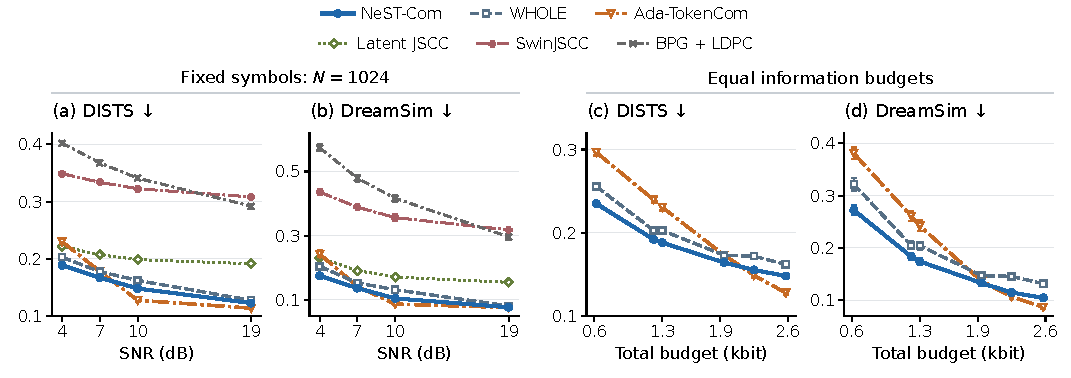
\includegraphics[width=\linewidth]{figure2.pdf}
\caption{Source-referenced reconstruction on common500. (a,b) Seven systems at $N=1024$, averaging three channel outcomes per source including failures. (c,d) Error-free equal-information budgets, including 57 shared overhead bits and Ada's additional 10-bit class; WHOLE/NeST share ceiling $(10,0)$. Points and bars are equal-source means and pointwise 95\% source-bootstrap intervals. Ada is the predicted-class fixed-frame adaptation. Lower values are favorable.}
\label{fig:performance}\end{figure*}
\fi
\subsection{Prefix-Constrained Reconstruction}
Invalid profile CRC/catalogue, body CRC, declared length, known padding, or arithmetic parsing yields a fixed gray image, as does valid NULL reception. Otherwise, RX decodes the actual prefix using the shared CDFs. At $e=(10,0)$, all maps are received and directly decoded. For an incomplete prefix, RX applies VAR's known-token overwrite and recursive state update~\cite{var}. It predicts the boundary map by argmax conditioned on complete received maps, then overwrites received positions:
\begin{equation}
\tilde q_{m+1,i}=\begin{cases}\hat q_{m+1,i},&i\leq K,\\q^{\mathrm{pred}}_{m+1,i},&i>K.\end{cases}
\label{eq:overwrite}
\end{equation}
Received boundary tokens serve two roles: they correct the residual representation and, through the merged boundary map, condition finer-scale prediction. Unreceived boundary positions retain their original coarse-conditioned prediction; there is no same-scale prediction loop. Complete received maps remain unchanged. After generating the finer maps,
\begin{equation}
\hat x=\Dc\!\left(\sum_{s=1}^{10}C_s(\tilde q_s)\right).
\label{eq:reconstruction}
\end{equation}
At the last scale, overwrite only changes the residual contribution.
